\documentclass[../sparc.tex]{subfiles}
\graphicspath{{\subfix{../images/}}}
\begin{document}

%%%%%%%%%%%%%%%%%%%%%%%%%%%%%%%%%%%%%%%%%%%%%%%%%%%%%%%%%%%%%%%%%%%%%%%%%%%%%%%%
\section{ЖК-дисплей}
\index{Разработка игр!Дисплей}

Для вывода информации мы будем использовать \emph{жидкокристаллический дисплей}
(ЖК-дисплей), подключаемый к Arduino.  Принцип работы данных дисплеев аналогичен
обычным ЖК-дисплеям, которые выводят информацию на вашем компьютере.  Более
конкретно мы будем использовать \emph{текстовый} ЖК-дисплей, который
предназначен для вывода текстовых символов.

На текстовых ЖК-дисплеях, экран поделён на клетки, внутри каждой из которых
можно отрисовать один символ (букву, знак препинания, цифру, или просто
какую-либо картинку.)  Между клетками обычно находится расстояние в один
пиксель.  Подобные дисплеи плохо подходят для отрисовки произвольных
изображений, тем не менее, некоторый простор для творчества у нас имеется.

Несмотря на свойства дисплея, которые на первый взгляд кажутся слишком
ограничивающими для наших задач, используя наше мастерство и творческий подход,
мы можем добиться достаточно интересных результатов в плане разработки игр.

Рабочая область дисплея 16x2 (16 столбцов, 2 строки) схематически выглядит, как
показано на рис. \ref{fig:lcd-16x2-schematics}.

\begin{figure}[ht]
  \centering
  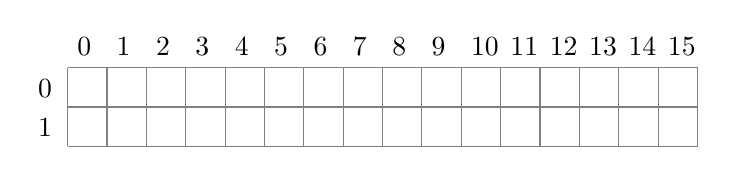
\begin{tikzpicture}
    \draw[gray, step=0.5] (0, 0) grid (8, 1);
    \foreach [count=\i from 0] \x in {0.0, 0.5, 1.0, ..., 7.5} {
      \draw (\x, 1.5) node[anchor=north west] {\i};
    }
    \foreach [count=\i from 0] \y in {0.5, 0.0} {
      \draw (-0.5, \y) node[anchor=south west] {\i};
    }
  \end{tikzpicture}
  \caption{Схематическое изображение дисплея 16x2 (16 столбцов, 2 строки.)}
  \label{fig:lcd-16x2-schematics}
\end{figure}

Внешний вид ЖК-дисплея 16x2 схематически показан на рис. \ref{fig:lcd-16x2}.

\begin{figure}[h]
  \centering
  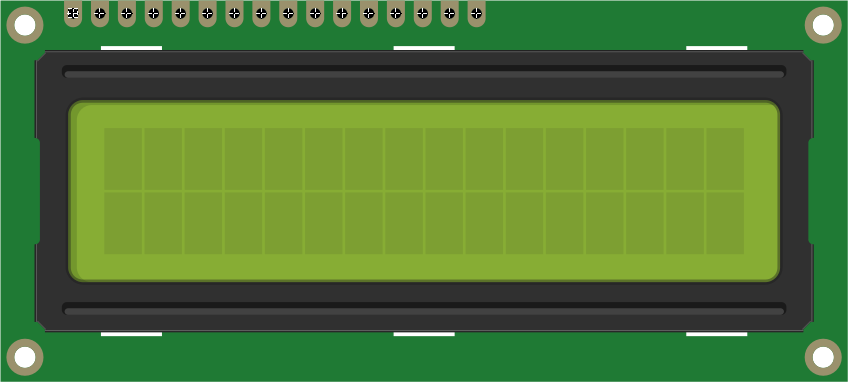
\includegraphics[width=10cm]{lcd-16x2}
  \caption{Схематическое изображение внешнего вида ЖК-дисплея 16x2 (источник
    изображения: набор электронных компонентов программы Fritzing.)}
  \label{fig:lcd-16x2}
\end{figure}

По возможности рекомендуется использовать для проектов, предложенных в данной
главе, ЖК-дисплей размером 20x4 (20 столбцов, 4 строки) Рабочая область
подобного дисплея больше (как показано на рис. \ref{fig:lcd-20x4-schematics}),
что позволяет реализовать более сложные игры.

\begin{figure}[ht]
  \centering
  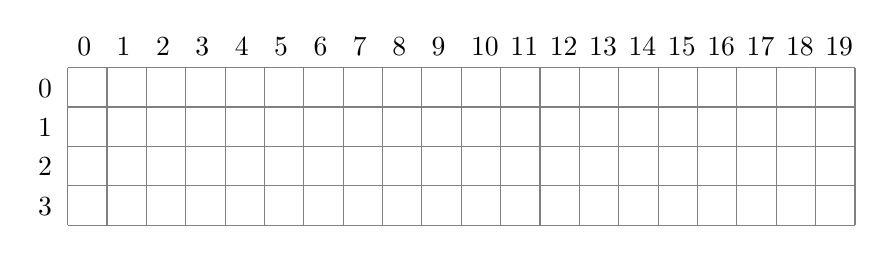
\begin{tikzpicture}
    \draw[gray, step=0.5] (0, 0) grid (10, 2);
    \foreach [count=\i from 0] \x in {0.0, 0.5, 1.0, ..., 9.5} {
      \draw (\x, 2.5) node[anchor=north west] {\i};
    }
    \foreach [count=\i from 0] \y in {1.5, 1.0, ..., 0.0} {
      \draw (-0.5, \y) node[anchor=south west] {\i};
    }
  \end{tikzpicture}
  \caption{Схематическое изображение дисплея 20x4 (20 столбцов, 4 строки.)}
  \label{fig:lcd-20x4-schematics}
\end{figure}

Внешний вид ЖК-дисплея 20x4 схематически показан на рис. \ref{fig:lcd-20x4}.

\begin{figure}[h]
  \centering
  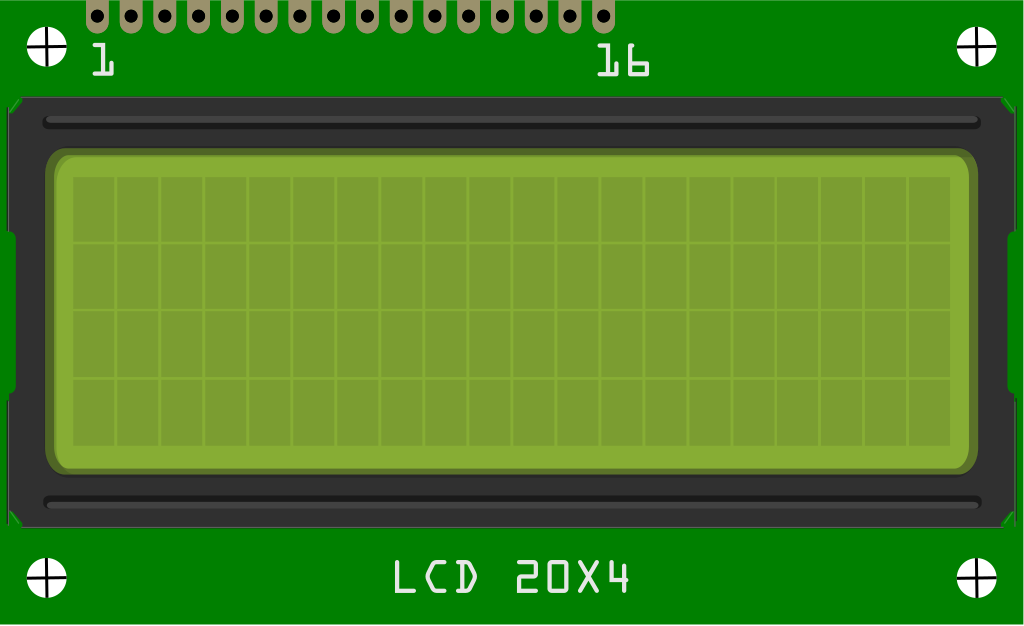
\includegraphics[width=10cm]{lcd-20x4}
  \caption{Схематическое изображение внешнего вида ЖК-дисплея 20x4 (источник
    изображения:
    \url{https://commons.wikimedia.org/wiki/File:LCD_20x4_breadboard.svg}.)}
  \label{fig:lcd-20x4}
\end{figure}

%%%%%%%%%%%%%%%%%%%%%%%%%%%%%%%%%%%%%%%%%%%%%%%%%%%%%%%%%%%%%%%%%%%%%%%%%%%%%%%%
\subsection{Подключение дисплея}
\index{Электроника!ЖК-дисплей}

Для упрощения нашей работы мы будем использовать ЖК-дисплей с интерфейсом
передачи данных, который называется \gls{I2C} (читается ``ай-ту-си''.)

Подробно об I2C будет сказано в следующем дополнительном подразделе.

Сейчас же, не вдаваясь в подробности можно сказать, что данный вариант
подключения требует всего 4 провода: питание, земля и две линии передачи данных.

Сам модуль I2C часто уже припаян к дисплею, но может идти и отдельно.  В случае
отдельного модуля, подключение выглядит, как на рис. \ref{fig:lcd-00}.

\begin{figure}[H]
  \centering
  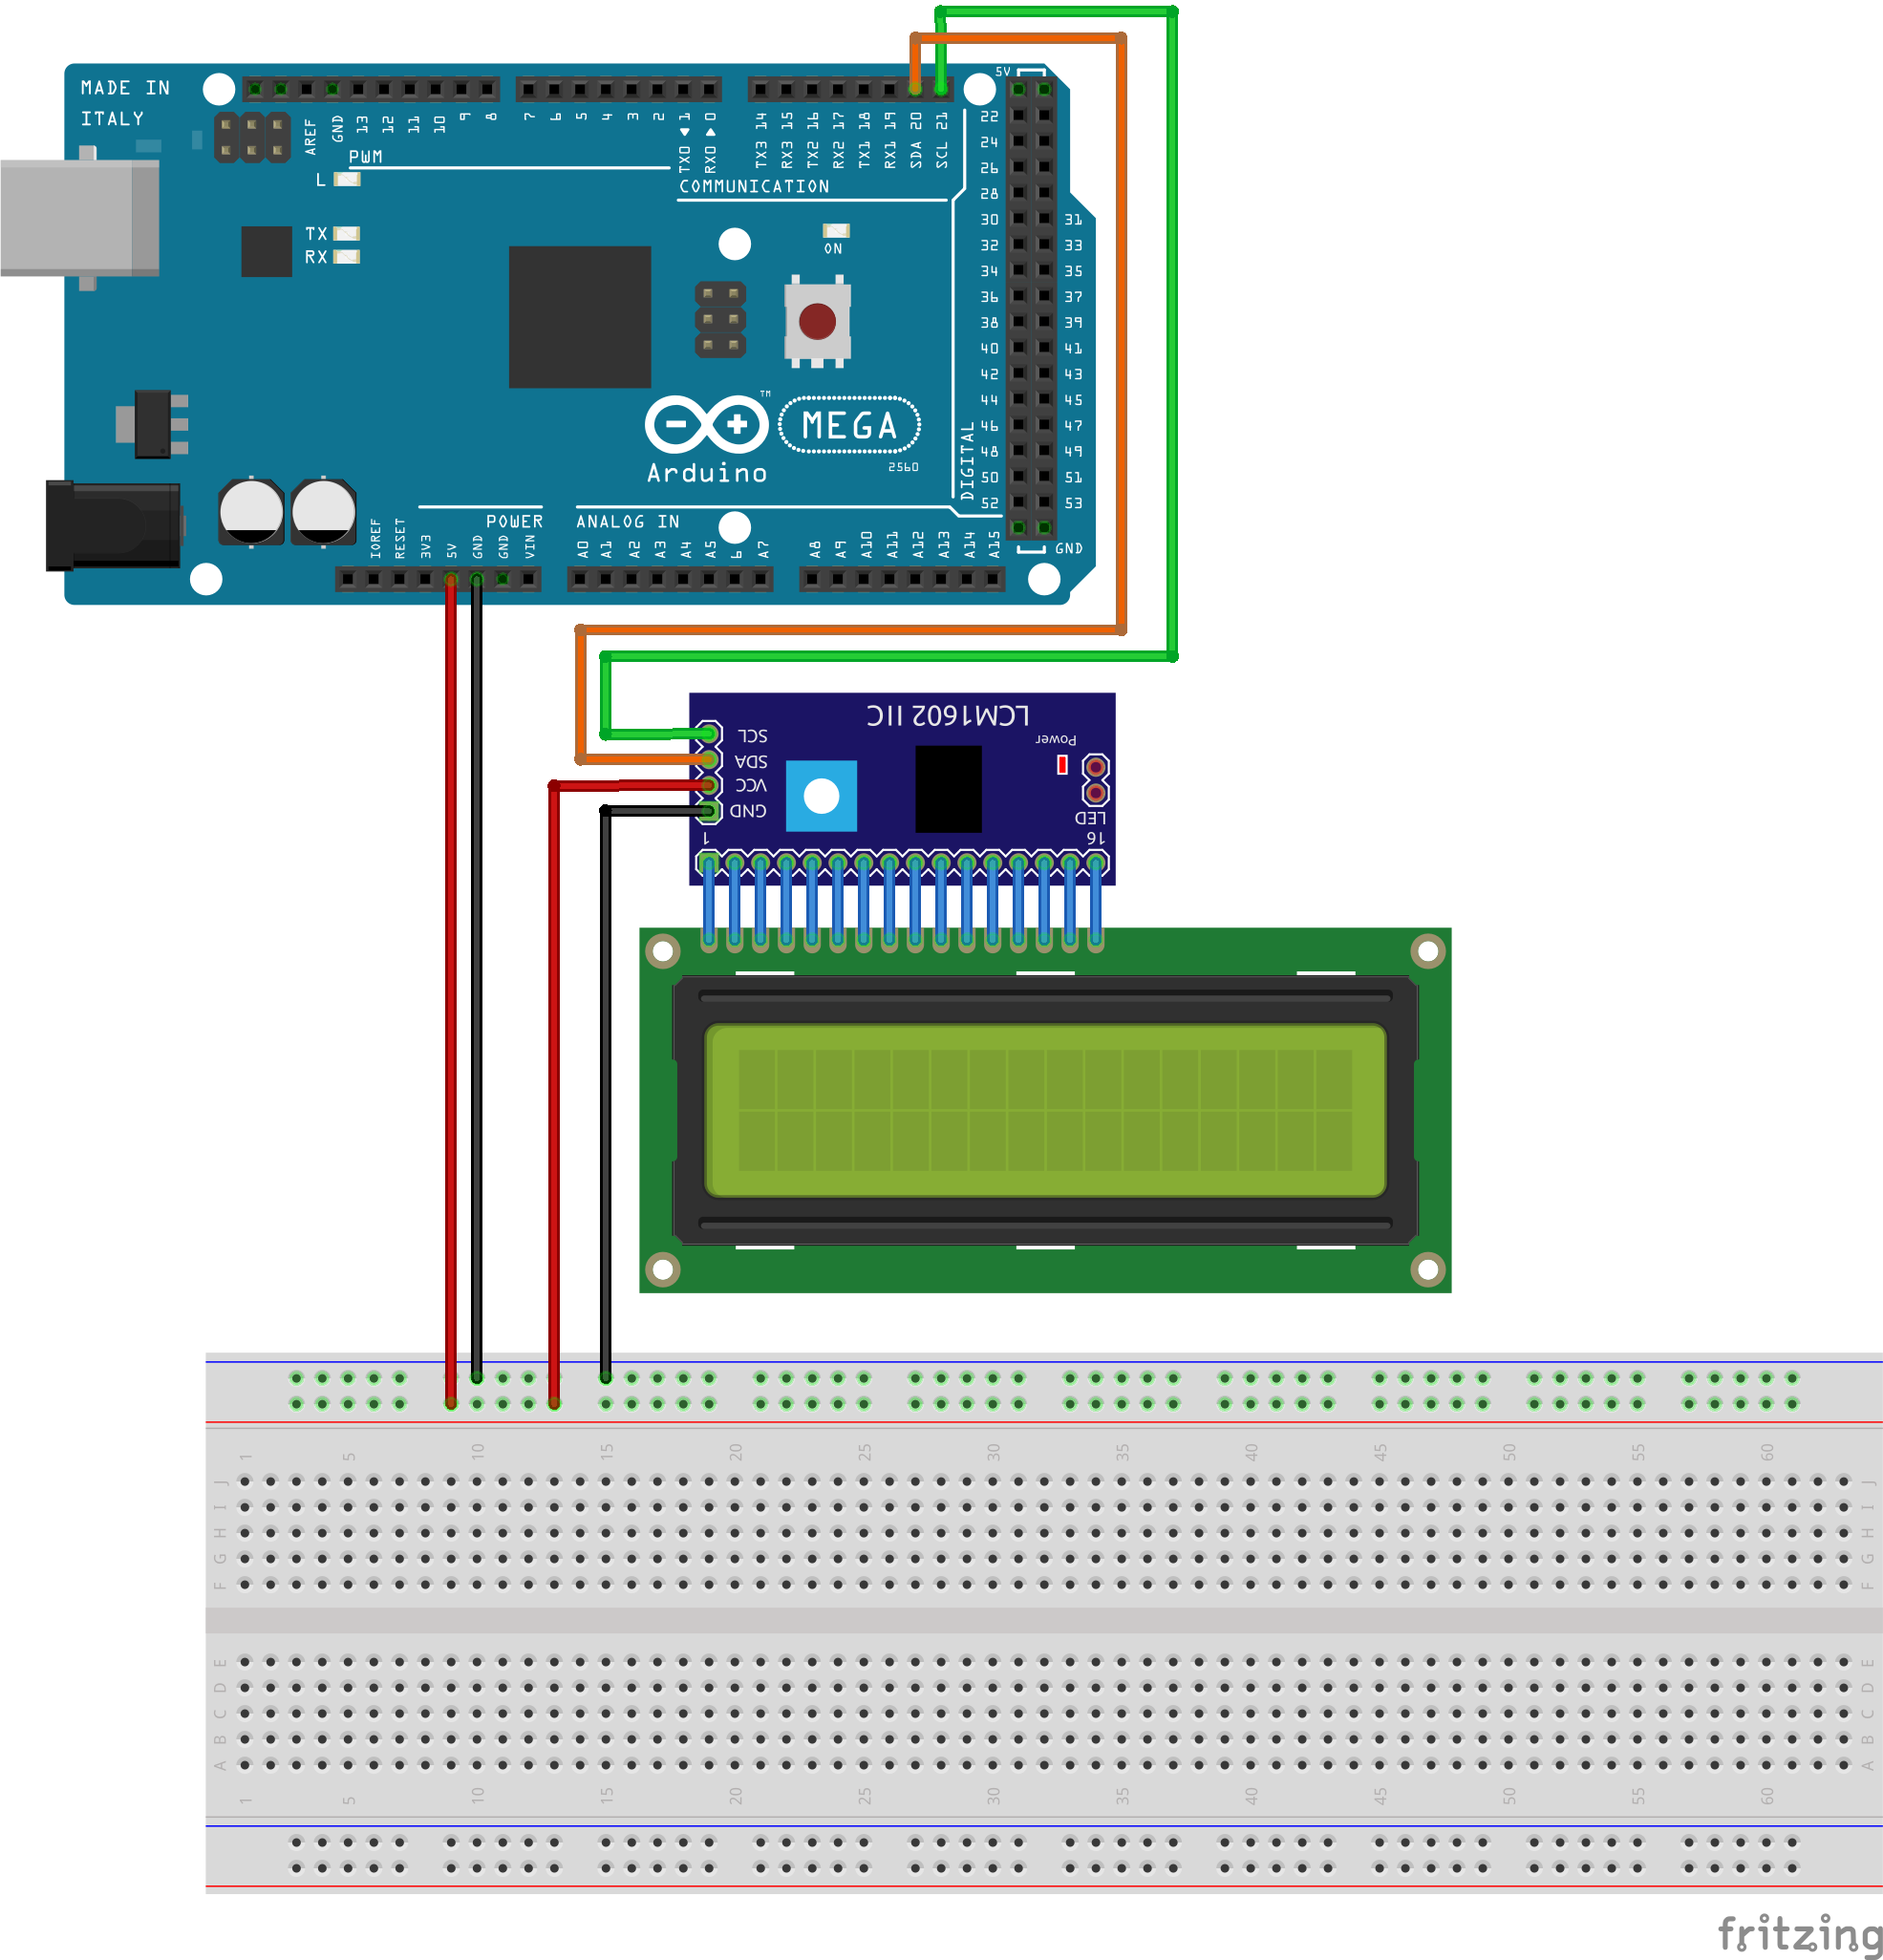
\includegraphics[width=12cm]{schematics/lcd-00}
  \caption{Схема подключения ЖК-дисплея 16x2 по интерфейсу I2C к Arduino Mega
    2560.}
  \label{fig:lcd-00}
\end{figure}

%%%%%%%%%%%%%%%%%%%%%%%%%%%%%%%%%%%%%%%%%%%%%%%%%%%%%%%%%%%%%%%%%%%%%%%%%%%%%%%%
\subsection{Вывод текста}
\index{Разработка игр!Вывод текста}

\newglossaryentry{LCD}{name=LCD, description={Liquid Crystal Display --
    Жидкокристаллический дисплей}}

Согласно традиции, первая программа, которую мы выведем -- это ``Привет, Мир!''.
Однако поскольку вывод русского текста на большинстве дисплеев организован
сложнее, нежели чем латиницы, то мы будем выводить ``Hello, World!''.

Для этого нам необходимо, во-первых, установить библиотеку для работы с
дисплеем; во-вторых, настроить дисплей на нужный режим работы, и только после
этого мы сможем вывести текст.

Начнём со скачивания библиотеки.  Проще всего это сделать через менеджер
библиотек, доступный из меню ``Инструменты'' (``Tools'') $\rightarrow$ ``Менеджер
библиотек'' (``Manage Libraries...''), далее в списке выбираем нужную библиотеку
и нажимаем на кнопку ``Установить'' (``Install''.)  Существуют несколько
библиотек, которые могут обеспечить работу ЖК-дисплея по протокола \gls{I2C}.
Мы можем взять библиотеку ``Liquid Crystal I2C'' версии 1.1.1 под авторством
Марко Шварца (Marco Schwartz).

Установив библиотеку, мы сможем использовать её функционал.

Первым делом в коде нам необходимо подключить библиотеку
``LiquidCrystal\_I2C.h'' -- это делается через специальную команду
\texttt{\#include}.

\begin{minted}{cpp}
#include <LiquidCrystal_I2C.h>
\end{minted}

В глобальной области кода (до функции \texttt{setup} и \texttt{loop}) необходимо
создать специальную переменную, через которую мы будем работать с дисплеем. Эта
переменная отличается от того, что мы видели раннее -- в данной переменной
хранится не число, а ссылка более сложный \emph{объект}\footnote{Термин
``объект'' относится к методологии программирования, которая называется
\emph{объектно-ориентированное программирование} (сокращённо ``ООП''.)  Мы пока
не будем заострять наше внимание на теме ООП, но любознательный читатель может
получить общее представление о данной методологии, например, из соответствующей
статьи в Wikipedia.}, который располагается где-то в памяти при работе программы
внутри микроконтроллера.

Назовём переменную \texttt{lcd}, по сокращению \gls{LCD} -- ``Liquid Crystal
Display'':

\begin{minted}{cpp}
LiquidCrystal_I2C lcd(0x27,  16, 2);
\end{minted}

Далее в функции \texttt{setup} необходимо выполнить настройку дисплея.

\begin{minted}{cpp}
lcd.init();
lcd.backlight();
\end{minted}

После этого уже в функции \texttt{loop} мы можем вывести текст.  Вывод текста,
как правило, делается в два этапа: во-первых, необходимо установить место, в
которое будет ``впечатан'' текст.  Для этого существует специальная функция
\texttt{setCursor}.

\begin{minted}{cpp}
lcd.setCursor(0, 0);
\end{minted}

Первый параметр \texttt{setCursor} задаёт позицию курсора по оси X, второй
параметр задаёт позицию по оси Y.

После этого наконец-то мы можем вывести текст.

\begin{minted}{cpp}
lcd.print("Hello, World!");
\end{minted}

Полностью код будет выглядеть примерно так, как показано ниже.

\begin{minted}{cpp}
#include <LiquidCrystal_I2C.h>

LiquidCrystal_I2C lcd(0x27,  16, 2);

void setup() {
  lcd.init();
  lcd.backlight();
}

void loop() {
  lcd.setCursor(0, 0);
  lcd.print("Hello, World!");
}
\end{minted}

При необходимости очистить экран можно ``затереть'' текст, впечатав поверх
пробелы, или же воспользоваться функцией \texttt{clear}, которая позволяет
очистить экран полностью.

%%%%%%%%%%%%%%%%%%%%%%%%%%%%%%%%%%%%%%%%%%%%%%%%%%%%%%%%%%%%%%%%%%%%%%%%%%%%%%%%
\subsubsection{Задачи}
\begin{enumerate}
\item Выровняйте тест по середине дисплея.
\item Сделайте так, чтобы текст мигал.
\item Разработайте ``Бегущую строку'', где текст будет перемещаться по экрану
  справа на лево.
\end{enumerate}

\end{document}
